\chapter{PLANNING OF WORK}

The basic implementation of this project will be done using prototype model and their will also be need to modify the structure of the project. Final flow of project will be fig. \ref{fig:finalflow}

\begin{figure}[H]
\centering
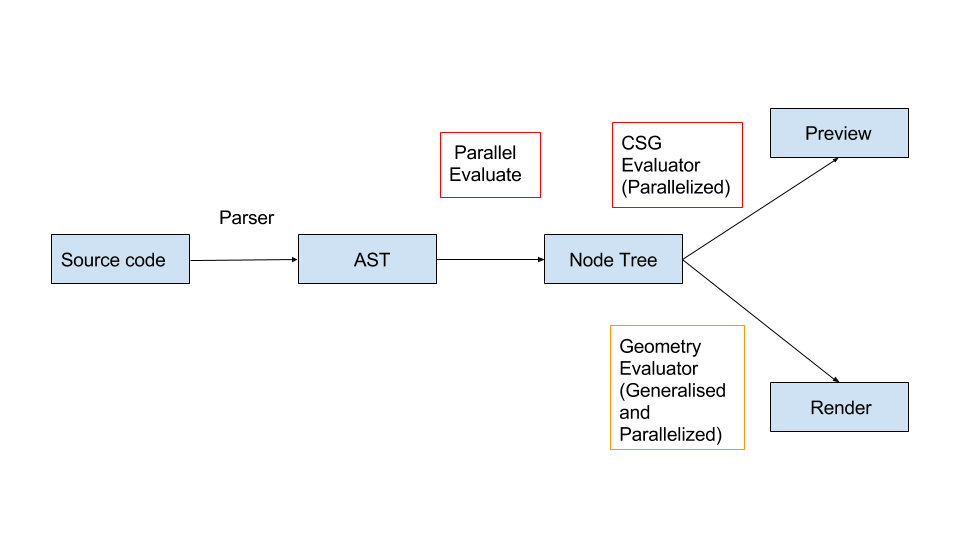
\includegraphics[width=\linewidth]{images/finalflow}
\caption{}
\label{fig:finalflow}
\end{figure}

\section{Steps of Implementation}
\begin{itemize}
	\item The first thing that needs to be done is understanding the flow of the software and figuring out what sections of code needs to be parallelized.
	\item After forming a firmer understanding of the problem, it will be required to check all the relevant data structures involved in evaluating the tree nodes. It will also be checked if any data structures used are needed to modified or not.
	\item After fixing the appropriate data structures, all the feasible and plausible approaches will be explored. Each approach will be evaluated on its merits and feasibility.
	\item Among all the options the one which is works well across all platform will be chosen. It goes without saying that the chosen solution must also meet all the requirement and implement the solution efficiently.
	\item After going through all of this the implementation will begin.
\end{itemize}
